\chapter{Introdução}

Observe abaixo a tabela da expectativa de vida no Brasil em 2008, segundo as regiões brasileiras (numeradas de 1 a 5) e gêneros (1 e 2). 

\begin{figure}[htb!]
  \centering
  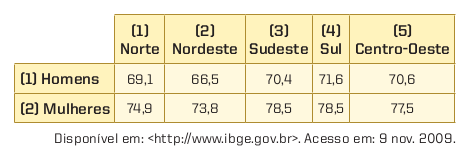
\includegraphics[width=.6\linewidth]{images/quadro.png}
  \caption{expectativa de vida brasileira em 2008}
  \label{fig:}
\end{figure}

Note que podemos encontrar a expectativa de vida de uma mulher residente na região Sul bastando olhar o cruzamento da linha 2 com a coluna 4, onde encontramos o valor de 78,5 anos. 

Em matemática, as tabelas como essa são chamadas de \textbf{matrizes}, sobre as quais definiremos a relação de igualdade e algumas operações. 


\section{Definição}
\dfn{Matriz}{Chama-se \textbf{matriz do tipo $m \times n$} (lemos ``m por n'') toda tabela de números dispostos em \textit{m} linhas e \textit{n} colunas.
} 

\begin{note}
  Essa tabela deve ser representada entre parênteses () ou entre colchetes [].
\end{note}

\ex{}{

  \begin{tasks}
    \task{
      $\begin{bmatrix}
        -6 & 7 \\
        -4 & 0 \\
        2 & -1 \\
      \end{bmatrix}$ 
      é uma matriz do tipo $3 \times 2$, pois tem 3 linhas e 2 colunas.
    }
    \task {
    $\begin{bmatrix}
      3 & \sqrt{2} & -5
    \end{bmatrix}$
    é uma matriz do tipo $1 \times 3$, pois tem 1 linha e 3 colunas.
    }
  \end{tasks}
}

\section{Representação genérica}

Indicamos por \textbf{$a_{ij}$} o elemento posicionado na linha \textit{i} e na coluna \textit{j} de uma matriz \textit{A}.

\ex{}{
  Na matriz:

  \begin{equation*}
    A_{3 \times 2} = \begin{bmatrix}
      6 & 7 \\
      -4 & 0 \\
      2 & -1
    \end{bmatrix}
  \end{equation*}

  \begin{itemize}
    \item o elemento 6 está na linha 1 e na coluna 1; por isso, ele é indicado por $a_{11}$, ou seja, $a_{11} = 6$;
    \item o elemento 7 está na linha 1 e na coluna 2; por isso, ele é indicado por $a_{12}$, ou seja, $a_{12} = 7$;
    \item analogamente, temos $a_{21} = -4$, $a_{22} = 0$, $a_{31} = 2$, $a_{32} = -1$.
  \end{itemize}


}

\dfn{Matriz Genérica}{
  Representamos genericamente uma matriz \textit{A} do tipo $m \times n$ da seguinte maneira:

  \begin{equation*}
    A_{m \times n} = \begin{bmatrix}
      a_{11} & a_{12} & a_{13} & \dots & a_{1n} \\
      a_{21} & a_{22} & a_{23} & \dots & a_{2n} \\
      \vdots & \vdots & \vdots & \vdots & \vdots \\
      a_{m1} & a_{m2} & a_{m3} & \dots & a_{mn} \\
    \end{bmatrix}
  \end{equation*}
}
  Como essa representação é muita extensa, vamos convencionar uma forma abreviada. Essa matriz pode ser representada simplesmente por 
  $A = (a_{ij})_{m \times n}$ ou, quando não houver possibilidade de confusão quanto ao tipo de matriz, por $A = (a_{ij})$.

\qs{}{Representar explicitamente a matriz $A = (a_{ij})_{2 \times 4}$ tal que $a_{ij} = 2i + j$.}

\sol{Primeiro, representamos genericamente a matriz \textit{A}, do tipo $2 \times 4$:
  \begin{equation*}
    A = \begin{bmatrix}
      a_{11} & a_{12} & a_{13} & a_{14} \\
      a_{21} & a_{22} & a_{23} & a_{24} \\
    \end{bmatrix}
  \end{equation*}

  A seguir, calculamos o valor de cada elemento $a_{ij}$, pela lei $a_{ij} = 2i + j$:

  \begin{tasks}(2)
    \task[] $a_{11} = 2 \cdot 1 + 1 = 3$
    \task[] $a_{12} = 2 \cdot 1 + 2 = 4$
    \task[] $a_{13} = 2 \cdot 1 + 3 = 5$
    \task[] $a_{14} = 2 \cdot 1 + 4 = 6$
    \task[] $a_{21} = 2 \cdot 2 + 1 = 5$
    \task[] $a_{22} = 2 \cdot 2 + 2 = 6$
    \task[] $a_{23} = 2 \cdot 2 + 3 = 7$
    \task[] $a_{24} = 2 \cdot 2 + 4 = 8$
  \end{tasks}

  Concluindo, temos a matriz: $A = \begin{bmatrix}
    3 & 4 & 5 & 6 \\
    5 & 6 & 7 & 8
  \end{bmatrix}$
}

\section{Matrizes Especiais}

\subsection{Matriz Quadrada}

\dfn{Matriz Quadrada}{É toda matriz cujo número de linhas é igual ao número de colunas.}

\begin{note}
  O número de linhas ou de colunas de uma matriz quadrada é chamado de \textbf{ordem} da matriz.
\end{note}

\ex{}{

  \begin{tasks}
    \task $\begin{bmatrix}
      4 & 9 & 0 \\
      -6 & 2 & 4 \\
      3 & 5 & -2
    \end{bmatrix}$
    é uma matriz quadrada de ordem 3.

    \task $\begin{bmatrix}
      3 & -9 \\
      0 & 1
    \end{bmatrix}$
    é uma matriz quadrada de ordem 2.
  \end{tasks}
}

Numa matriz A de ordem \textit{n}, os elementos $a_{ij}$, tais que $i = j$ formam a \textbf{diagonal principal} da matriz, e os elementos 
$a_{ij}$, tais que $i + j = n + 1$ formam a \textbf{diagonal secundária}. Por exemplo:

\begin{figure}[htb!]
  \centering
  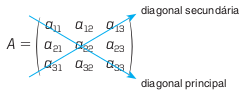
\includegraphics[width=.3\linewidth]{images/quadrada.png}
\end{figure}

\subsection{Matriz Identidade}

\dfn{Matriz Identidade}{É a matriz quadrada cujos elementos da \textbf{diagonal principal} são iguais a 1 e os demais iguais a 0.}

Indicamos por $I_n$ a matriz identidade de ordem \textit{n}.

\ex{}{
  \begin{tasks}
    \task $I_3 = \begin{bmatrix}
      1 & 0 & 0 \\
      0 & 1 & 0 \\
      0 & 0 & 1
    \end{bmatrix}$

    \task $I_2 = \begin{bmatrix}
      1 & 0 \\
      0 & 1
    \end{bmatrix}$
  \end{tasks}
}

\subsection{Matriz Nula}

\dfn{Matriz Nula}{É a matriz que possui todos os elementos iguais a zero.}

\ex{}{
  \begin{tasks}
    \task 
  $\begin{bmatrix}
    0 & 0 & 0 \\
    0 & 0 & 0 \\
    0 & 0 & 0 \\
  \end{bmatrix}$
  \task $\begin{bmatrix}
    0 & 0 \\
    0 & 0 \\
  \end{bmatrix}$
  \end{tasks}
}

\subsection{Transposta de uma Matriz}

\dfn{Transposta de uma Matriz}{Transposta de uma matriz \textit{A} é a matriz $A^t$ tal que os números que a formam são obtidos através da troca de posição entre linhas e colunas da matriz \textit{A}. }

